\documentclass{../notes}

\title{高等运作管理 HW03}

\begin{document}
    \maketitle
    \paragraph*{1}

    根据$(Q, R)$策略,有

    \begin{equation}
        \begin{aligned}
            \alpha &= F(Q) \\
            \beta &= 1 - \frac{n(R)}{\mu}
        \end{aligned}
    \end{equation}

    \begin{subquestions}
        \item 由于$D\sim N(100, 50^2)$,则有

        \begin{equation}
            \begin{aligned}
                \alpha &= F(R) = \Phi\left(\frac{R - \mu}{\sigma}\right) \\
                &= \Phi(0.7) = 0.758 \\
                \beta &= 1 - \frac{n(R)}{Q} \\
                &= 1 - \frac{\sigma\left[f\left(\frac{R-\mu}{\sigma}\right) - \frac{R-\mu}{\sigma}\left(1 - \Phi\left(\frac{R-\mu}{\sigma}\right)\right)\right]}{Q} \\
                &= 0.964
            \end{aligned}
        \end{equation}
        \item 由于均匀分布$U(a, b)$的均值为$(a + b) / 2$,方差为$(a^2 + ab + b^2)/3$,得到$a=100-50\sqrt3, b=100+50\sqrt 3$,则

        \begin{equation}
            \begin{aligned}
                \alpha &= F(R) = \frac{R-a}{b-a} = 0.702 \\
                \beta &= 1 - n(R)/\mu = \frac{1}{\mu}\int_R^\infty \frac{(x-R)}{b-a} \dd x \\
                &= 0.962
            \end{aligned}
        \end{equation}
    \end{subquestions}

    \paragraph*{2}

    \begin{subquestions}
        \item 首先计算当提前期未改变时的服务水平和库存水平。每四周的需求分布为$D^{(4)}\sim N(4\times 200, 4\times 50^2), \mu^{(4)} = 800, \sigma^{(4)} = 100$。

        \textbf{服务水平$\beta$:}

        \begin{equation}
            \begin{aligned}
                z^{(4)} &= \frac{R-\mu^{(4)}}{\sigma^{(4)}} = 0.5 \\
                \beta^{(4)} &= 1 - \frac{n(R)}{Q} \\
                &= 1 - \frac{\sigma\left[\phi(z) - z\left(1 - \Phi(z)\right)\right]}{Q} \\
                &= 0.967
            \end{aligned}
        \end{equation}

        \textbf{库存水平$E\left(\mathrm {IL}^{(4)}\right)$:}

        \begin{derive}[E\left(\mathrm{IL}^{(4)}\right)]
            &= \int_0^{Q+R} xf_{\mathrm {IL}^{(4)}}(x) \dd x \\
            &= \int_0^{Q+R} \frac{x}{Q}\int_{R}^{Q+R} \phi\left(\frac{(u-x)-\mu^{(4)}}{\sigma^{(4)}}\right) \dd u\dd x \\
            &= 351.7
        \end{derive}

        再计算提前期改变后的服务水平和库存水平。每两周的需求分布为$D^{(2)}\sim N(2\times 200, 2\times 50^2), \mu^{(2)} = 400, \sigma^{(2)} = 50\sqrt 2$。

        \textbf{服务水平$\beta$:}

        \begin{equation}
            \begin{aligned}
                z^{(2)} &= \frac{R - \mu}{\sigma} = 6.36 \\
                \beta^{(2)} &= 1 - \frac{n(R)}{Q} \\
                &= 1 - \frac{\sigma\left[\phi(z) - z\left(1 - \Phi(z)\right)\right]}{Q} \\
                &\approx 1
            \end{aligned}
        \end{equation}

        \textbf{库存水平$E\left(\mathrm {IL}^{(2)}\right)$:}

        \begin{derive}[E\left(\mathrm{IL}^{(2)}\right)]
            &\approx \frac{Q}{2} + R - \mu^{(2)} \\
            &= 750
        \end{derive}

        \item 当保持$Q, \beta$不变时,有

        \begin{equation}
            \int_R ^\infty (x-R)f(x) \dd x = n(R) = Q(1 - \beta) = 19.8
        \end{equation}

        解得$R = 419$,$E\left(\mathrm{IL}^{(2)}\right)\approx \frac{Q}{2} + R - \mu^{(2)}=319$
    \end{subquestions}

    \paragraph*{3} 当每个区域单独销售时,有$D^{(2)}\sim N\left(2\times 25, 2\times 5^2\right)$,每个销售点所需的安全库存(式中$\Phi^{-1}$为$\Phi$的反函数)

    \begin{equation}
        \mathrm {SS}_{0} = \Phi^{-1}(\alpha) \sigma = 9.06
    \end{equation}

    因此所需的安全库存为$9.04\times 4 = 36.25$

    当集中销售时,有$D^{(8)} = \sim N\left(8\times 25, 8\times 5^2\right)$

    \begin{equation}
        \mathrm {SS}_{0} = \Phi^{-1}(\alpha) \sigma = 18.12
    \end{equation}

    所需的安全库存为单独销售时安全库存的一半。

    对于相关性的定性分析

    \begin{enumerate}
        \item[$\rho > 0$] 当$\rho > 0$时,集中需求后整体面临的需求波动更大,因此在$\alpha$不变的前提下,需要更多的安全库存以应对需求的波动。极端情况下,$\rho = 1$时,集中需求和不集中需求完全相同,库存集成对降低安全库存没有帮助。
        \item[$\rho < 0$] 反之,当$\rho < 0$时,集中需求后整体面临的需求波动相较于独立时更小,因此所需的安全库存也更小。极端情况下,$\rho = -1$时,集中需求后需求为常数,不需要安全库存。
    \end{enumerate}

    \paragraph*{4} 使用一个仓库同时管理四个销售点的库存,每个销售点仅维持较低水平的库存,当需要额外的库存时,再从仓库调度新的库存。

    \paragraph*{5}

    \begin{subquestions}
        \item \label{5.a} $P(\mathrm{IL} = i) = P(D = S - i) = \frac{(\lambda \tau)^{(S-i)}}{(S-i)!}e^{-\lambda\tau}$

        此时,持有成本与缺货成本为

        \begin{equation}
            \begin{aligned}
                E(C_o) &= h\int_{S-1}^S E\left(y - D\right)^+\dd y \\
                E(C_u) &= p\int_{S-1}^S E\left(D-y\right)^+\dd y
            \end{aligned}
        \end{equation}

        \item 库存水平的状态转移图如图\ref{fig:5-1}所示

        \begin{figure}[h]
            \centering
            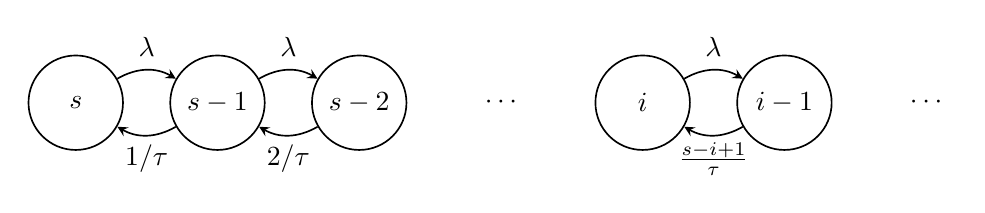
\begin{tikzpicture}
                [
                    Node/.style={circle, draw=black, minimum size=12mm, semithick},
                    EmptyNode/.style={circle, draw=white},
                    Connection/.style={semithick, -stealth, draw=black}
                ]
                \node[Node] (S) at (0, 0) {$s$};
                \node[Node, right of=S, xshift=0.8cm] (S-1) {$s-1$};
                \node[Node, right of=S-1, xshift=0.8cm] (S-2) {$s-2$};
                \node[EmptyNode, right of=S-2, xshift=0.8cm] (gap1) {$\cdots$};
                \node[Node, right of=gap1, xshift=0.8cm] (i) {$i$};
                \node[Node, right of=i, xshift=0.8cm] (i-1) {$i-1$};
                \node[EmptyNode, right of=i-1, xshift=0.8cm] (gap2) {$\cdots$};

                \path[Connection] (S) to[bend left=30] node[yshift=0.3cm] {$\lambda$} (S-1);
                \path[Connection] (S-1) to[bend left=30] node[yshift=0.3cm] {$\lambda$} (S-2);
                \path[Connection] (i) to[bend left=30] node[yshift=0.3cm] {$\lambda$} (i-1);

                \path[Connection] (S-1) to[bend left=30] node[yshift=-0.3cm] {$1 / \tau$} (S);
                \path[Connection] (S-2) to[bend left=30] node[yshift=-0.3cm] {$2 / \tau$} (S-1);
                \path[Connection] (i-1) to[bend left=30] node[yshift=-0.3cm] {$\frac{s - i + 1}{\tau}$} (i);
            \end{tikzpicture}

            \caption{允许延期交货时库存水平的状态转移图}
            \label{fig:5-1}
        \end{figure}

        根据状态转移图,对于每个状态$i < S$,有

        \begin{equation}
            \left(\lambda + \frac{S-i}{\tau}\right)P(\mathrm{IL} = i) = \lambda P(\mathrm{IL} = i+1) + \frac{s - i + 1}{\tau}P(\mathrm{IL} = i-1)
        \end{equation}

        特别地,当$i=S$时,有

        \begin{equation}
            \lambda P(\mathrm {IL} = S) = \frac{1}{\tau} P(\mathrm {IL} = S-1)
        \end{equation}

        解得

        \begin{equation}
            \begin{aligned}
                P(\mathrm {IL} = S) &= e^{-\lambda \tau} \\
                P(\mathrm {IL} = i) &= \frac{(\lambda \tau)^{(S-i)}}{(S-i)!}P(\mathrm {IL}= S) = \frac{(\lambda \tau)^{(S-i)}}{(S-i)!}e^{-\lambda \tau}
            \end{aligned}
        \end{equation}

        与\ref{5.a}中结果相同,表明库存水平的概率分布与提前期的分布无关。

        \item 库存水平的状态转移图如图\ref{fig:5-2}所示

        \begin{figure}[h]
            \centering
            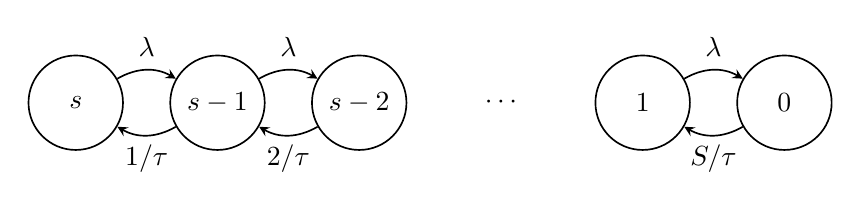
\begin{tikzpicture}
                [
                    Node/.style={circle, draw=black, minimum size=12mm, semithick},
                    EmptyNode/.style={circle, draw=white},
                    Connection/.style={semithick, -stealth, draw=black}
                ]
                \node[Node] (S) at (0, 0) {$s$};
                \node[Node, right of=S, xshift=0.8cm] (S-1) {$s-1$};
                \node[Node, right of=S-1, xshift=0.8cm] (S-2) {$s-2$};
                \node[EmptyNode, right of=S-2, xshift=0.8cm] (gap1) {$\cdots$};
                \node[Node, right of=gap1, xshift=0.8cm] (1) {$1$};
                \node[Node, right of=1, xshift=0.8cm] (0) {$0$};

                \path[Connection] (S) to[bend left=30] node[yshift=0.3cm] {$\lambda$} (S-1);
                \path[Connection] (S-1) to[bend left=30] node[yshift=0.3cm] {$\lambda$} (S-2);
                \path[Connection] (1) to[bend left=30] node[yshift=0.3cm] {$\lambda$} (0);

                \path[Connection] (S-1) to[bend left=30] node[yshift=-0.3cm] {$1 / \tau$} (S);
                \path[Connection] (S-2) to[bend left=30] node[yshift=-0.3cm] {$2 / \tau$} (S-1);
                \path[Connection] (0) to[bend left=30] node[yshift=-0.3cm] {$S / \tau$} (1);
            \end{tikzpicture}

            \caption{不允许延期交货时库存水平的状态转移图}
            \label{fig:5-2}
        \end{figure}

        根据状态转移图,对于每个状态$i < S$,有

        \begin{equation}
            \left(\lambda + \frac{S-i}{\tau}\right)P(\mathrm{IL} = i) = \lambda P(\mathrm{IL} = i+1) + \frac{s - i + 1}{\tau}P(\mathrm{IL} = i-1)
        \end{equation}

        特别地,当$i=S$与$i=0$时,有

        \begin{equation}
            \begin{aligned}
                \lambda P(\mathrm {IL} = S) &= \frac{1}{\tau} P(\mathrm {IL} = S-1) \\
                \lambda P(\mathrm {IL} = 1) &= \frac{S}{\tau} P(\mathrm {IL} = 0)
            \end{aligned}
        \end{equation}

        解得

        \begin{equation}
            \begin{aligned}
                P(\mathrm {IL} = S) &= \frac{1}{1 + \sum_{k=1}^S k!(\tau\lambda)^k} \\
                P(\mathrm {IL} = i) &= \frac{(\lambda\tau)^{(S-i)}}{(S-i)!\left(1 + \sum_{k=1}^S k!(\tau\lambda)^k\right)}
            \end{aligned}
        \end{equation}
    \end{subquestions}

    \paragraph*{6} Consider a system with the following data:

    \begin{equation*}
        L_1 = L_2 = 5, \mu = 10, \sigma = 5, e_1 = 0.5, e_2 = 1, b_1 = 10
    \end{equation*}

    Assume that $L_2 = 0$ instead of $5$.

    \begin{subquestions}
        \item \label{6.1} 已知,单个周期内的需求$D\sim N(10, 5^2)$

        对于第一级:$L_1 + 1 = 6$个周期内的需求分布为$D^{(6)} \sim N(6\times 10, 6\times 5^2)$,设其分布函数为$F^{(6)}: \R\rightarrow [0, 1]$,则

        \begin{equation}
            F^{(6)} \left(\hat S_1^*\right) = \frac{e_2 + b_1}{e_1 + e_2 + b_1}
        \end{equation}

        解得$\hat S_1^* = 81$,进一步得到$\hat C_1\left(\hat S_1^*\right) = -47$

        对于第二级:$L_2 = 5$个周期内的需求分布为$D^{(5)}\sim N(5\times 10, 5\times 5^2)$,则有

        \begin{equation}
            \hat C_2\left(\hat S_2\right) = h_2\left(\hat S_2 - \mu_2\right) + \hat C_1\left(\hat S_1^*\right)+\int_{\hat S_2 - \hat S_1^*}^{\infty} \frac{\left(\hat C_1\left(\hat S_2 - u\right) - \hat C_1\left(S_1^*\right)\right)\phi\left(\frac{u-\mu_2}{\sigma_2}\right)}{\sigma_2} \dd u
        \end{equation}

        解得$\hat S_2^* = 129.7, \hat C_2\left(\hat S_2^*\right)=39.38$

        \item 当$L_2 = 0$时,由于$L_1$不变,则\ref{6.1}中$\hat S_1^* = 81$不变

        \begin{enumerate}[label=\arabic{*}.]
            \item 若$\hat S_2\geq \hat S_1^*$,此时有$\hat C_2\left(\hat S_2\right) = h_2\hat S_2 + \hat C_1\left(\hat S_1\right)$,而$\dd \hat C_2 / \dd \hat S_2 = h_2 > 0$,则$\hat S_2^* = \hat S_1^* = 81$
            \item 若$\hat S_2 < \hat S_1^*$,此时有$\hat C_2\left(\hat S_2\right) = h_2\hat S_2 + \hat C_1\left(\hat S_2\right)$,求导

            \begin{equation}
                \frac{\dd \hat C_2}{\dd \hat S_2} = h_2 + e_1 + \left(h_1 + b_1\right)\left[\Phi\left(\frac{\hat S_2 - \mu^{(6)}}{\sigma^{(6)}} - 1\right)\right] < 0
            \end{equation}

            因此,$\hat C_2\left(\hat S_2\right) > \hat C_2 \left(\hat S_1^*\right)$
        \end{enumerate}

        由此,$\hat S_2^* = 81$
    \end{subquestions}
\end{document}